\documentclass[aspectratio=169]{beamer}
\usepackage{amsmath, amssymb, amsfonts, mathtools}
\usepackage{booktabs, graphicx}
\usepackage{hyperref}
\usepackage{fontspec}
\usepackage{siunitx}
\usepackage{physics}
\usepackage{caption}
\usepackage{listings}
\usepackage{tikz}
\usepackage{multicol}
\usepackage{tabularx}
\usepackage{fontawesome}
% \usepackage{ulem}
\usetikzlibrary{arrows.meta,positioning,shapes,fit,calc}
\usepackage{pgfplots}
\pgfplotsset{compat=1.18}
  \newcommand{\E}{\mathbb{E}}
\newcommand{\Var}{\mathrm{Var}}
\definecolor{sb-bg}{HTML}{0B0F19}
\definecolor{sb-panel}{HTML}{121826}
\definecolor{sb-text}{HTML}{E6E6E6}
\definecolor{sb-accent}{HTML}{6EE7F9} % cyan
\definecolor{sb-accent2}{HTML}{A78BFA} % violet

%Для защит онлайн лучше использовать разрешение 16x9
%\documentclass[aspectratio=169]{beamer}

\input{preamble.tex}

% То, что в квадратных скобках, отображается внизу по центру каждого слайда.
\title[MyBudget]{умный помощник студента по личным финансам}
\subtitle{Инвест-питч и бизнес-план}

% То, что в квадратных скобках, отображается в левом нижнем углу.
\institute[СПбГУ]{Экономико-правовые основы рынка}

% То, что в квадратных скобках, отображается в левом нижнем углу.
\author[1 Команда]{группа 24.М71-мм}

\begin{document}
{
\setbeamertemplate{footline}{}
% Лого университета или организации, отображается в шапке титульного листа
\begin{frame}
  \includegraphics[width=1.4cm]{pictures/SPbGU_Logo.png}
\vspace{-35pt}
\hspace{-10pt}
\begin{center}
   \begin{tabular}{c}
        \scriptsize{Санкт-Петербургский государственный университет} \\
        \scriptsize{Кафедра системного программирования}
    \end{tabular}
\titlepage
\end{center}

\btVFill

{\scriptsize
  % У научного руководителя должна быть указана научная степень
   \textbf{Преподаватель:} Старший преподаватель М.Х. Немешев \\
 }
\begin{center}
  \vspace{5pt}
  \scriptsize{Санкт-Петербург\\
                 2025}
  \end{center}

\end{frame}
}

% ---------- Проблема ----------
\begin{frame}{Проблема}
  \begin{itemize}
    \item Нестабильные доходы (стипендия, подработка) и ограниченный бюджет.
    \item Отсутствие привычки учёта и накоплений — «дожить до конца месяца».
    \item Подписки и спонтанные траты «съедают» бюджет незаметно.
    \item Тяжёлые PFM-приложения ориентированы на взрослых пользователей.
  \end{itemize}
  \note{Подчеркнуть: существующие инструменты перегружены, студентам нужен простой, понятный помощник.}
\end{frame}

% ---------- Решение ----------
\begin{frame}{Решение: MyBudget}
  Простое приложение, которое:
  \begin{itemize}
    \item автоматизирует учёт доходов и расходов (категории, подсказки).
    \item прогнозирует, на сколько дней хватит средств.
    \item помогает ставить цели: ноутбук, поездка, подушка безопасности.
    \item даёт советы по правилам 50/30/20 и контролю подписок.
  \end{itemize}
  \note{Ключ — фраза «на сколько дней хватит», легко понимается и цепляет.}
\end{frame}



% ---------- Рынок и аудитория ----------
\begin{frame}{Аудитория}
  \begin{itemize}
    \item Студенты, 18–30 лет (Россия/СНГ).
    \item Доход до 50\,000 {\footnotesize \faRub}/мес.
    \item Смартфон Android/iOS.
    \item \textbf{Цель}: дисциплина расходов и накопления на краткосрочные цели.
  \end{itemize}
\end{frame}


% ---------- Slide 4: Конкуренты ----------
\begin{frame}{Анализ конкурентов}
  \begin{tabularx}{\linewidth}{@{} l X X @{}}
    \toprule
    \textbf{Приложение} & \textbf{Плюсы} & \textbf{Минусы для студента} \\
    \midrule
      CoinKeeper & Яркая визуализация, гибкие категории & Сложновато, нет простых советов \\
      ZenMoney & Синхронизация с банками & Дорогая подписка, избыточность \\
      Money Manager & Простота учёта & Слабые цели/советы, локализация \\
      MyBudget & Студент-центричность, простые советы, низкая цена & \textbf{—} \\
    \bottomrule
  \end{tabularx}
  \note{Сделать акцент на позиционировании: «про студентов и для студентов».}
\end{frame}



% ---------- Рынок ----------
\begin{frame}{Рынок: TAM / SAM / SOM}
  \begin{columns}[T,onlytextwidth]
    \column{0.65\textwidth}
    \begin{itemize}
      \item \textbf{TAM}: рынок приложений для управления личными финансами (Personal Finance Management, PFM) в РФ. Все пользователи приложений личных финансов.
      \item \textbf{SAM}: студенты и молодые специалисты — \~6 млн.
      \item \textbf{SOM}: достижимая доля 1\% за 2 года — \~60\,000 пользователей.
    \end{itemize}
    \column{0.35\textwidth}
    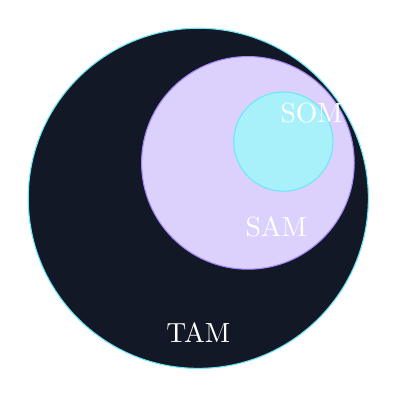
\begin{tikzpicture}[scale=0.9]
      \fill[sb-panel,draw=sb-accent] (0,0) circle (2.4);
      \fill[sb-accent2!40,draw=sb-accent2] (0.7,0.5) circle (1.5);
      \fill[sb-accent!60,draw=sb-accent] (1.2,0.8) circle (0.7);
      \node[white] at (0, -1.9) {TAM};
      \node[white] at (1.1, -0.4) {SAM};
      \node[white] at (1.6, 1.2) {SOM};
    \end{tikzpicture}
  \end{columns}
  \break
  \tiny
  TAM — \textit{Total Addressable Market} (весь потенциальный рынок).\\
  SAM — \textit{Serviceable Available Market} (достижимый сегмент).\\
  SOM — \textit{Serviceable Obtainable Market} (реально осваиваемый сегмент).
  \note{Числа ориентировочные для учёбы. При необходимости можно сослаться на отчёты финтех/аналитики.}
\end{frame}


% ---------------- Маркетинг-план ----------------
\begin{frame}{Маркетинг-план (6 месяцев)}
  \begin{columns}[T,onlytextwidth]
  \column{0.6\textwidth}
  \begin{enumerate}
    \item \textbf{Органика (1–3 мес)}: ВКонтакте/Telegram в вузах, финграмотность, короткие видео.
    \item \textbf{Партнёрства (4–6 мес)}: студенческие сообщества, скидки.
    \item \textbf{Рефералы}: бонусы за приглашения / streak-задачи.
    \item \textbf{Удержание}: еженедельные челленджи, push-уведомления, внутренняя геймификация.
  \end{enumerate}
  \vspace{0.3em}
  \textbf{KPI:} 15k установок, 30\% retention.
  \column{0.4\textwidth}
  \begin{block}{Мини-бюджет (6 мес)}
    \begin{itemize}
      \item Инфлюенсеры: 30k {\footnotesize \faRub} → 10k установок
      \item Университетские каналы: 10k {\footnotesize \faRub} → 5k установок
    \end{itemize}
    \textbf{Итого:} 40k {\footnotesize \faRub} → 15k установок
  \end{block}
  \end{columns}
\end{frame}


% ---------------- Monetization & Profit ----------------
\begin{frame}{Прибыльность}
  \begin{itemize}
    \item Freemium: бесплатный учёт + базовые советы.
    \item Premium 99 {\footnotesize \faRub}/мес: прогнозы, отчёты, цели, экспорт.
    \item Партнёрства: кэшбэк/скидки для студентов.
  \end{itemize}
  \vspace{0.6em}
  \begin{tabular}{@{} l r @{}}
  \toprule
  Пользователи через 1 год & 20,000 \\
  Конверсия в premium (5\%) & 1\,000 \\
  Месячная выручка & 99,000 {\footnotesize \faRub} \\
  Годовая выручка & 1.2 млн {\footnotesize \faRub} \\
  Затраты (серверы+маркетинг) & 300k {\footnotesize \faRub}/год \\
  \textbf{Годовая прибыль} & \textbf{\~900k {\footnotesize \faRub}} \\
  \bottomrule
  \end{tabular}
  \note{Пояснить, что это ориентир для учебной работы. Показывает экономическую достижимость.}
 \end{frame}



% ---------------- Mockups ----------------
\begin{frame}{Дизайн и интерфейс (mockups)}
  \begin{multicols}{2}
  \begin{itemize}
    \item Главный экран: баланс + совет дня.
    \item Диаграмма трат по категориям.
    \item Цель: «Новый ноутбук» с прогрессом.
  \end{itemize}
  \end{multicols}
  \vspace{0.5em}
  \begin{center}
  \includegraphics[width=0.6\linewidth]{economy/all.png}\hfill
  \end{center}
  \note{Если нет времени на демо, используем AI-картинки интерфейса в единой палитре.}
\end{frame}

% ---------------- Team ----------------
\begin{frame}{Команда}
  \begin{tabularx}{\linewidth}{@{} l l X @{}}
  \toprule
  \textbf{Имя} & \textbf{Роль} & \textbf{Навыки} \\
  \midrule
  Альшаеб Басель & Руководитель / Backend & Laravel, Spring Boot, архитектура API \\
  Малыгин Даниил Александрович & UI/UX дизайнер & Figma, прототипирование, дизайн-системы \\
  Макаров Павел Михайлович & Маркетинг & аналитика, партнёрства \\
  Малыгин Даниил Александрович & Мобильная разработка & Flutter / React Native \\
  \bottomrule
  \end{tabularx}
\end{frame}


% ---------------- Roadmap ----------------
\begin{frame}{Дорожная карта (6 месяцев)}
  \begin{enumerate}
    \item Проектирование и UX (1 мес)
    \item MVP: учёт + диаграммы (2 мес)
    \item Альфа-тест в вузах (1 мес)
    \item Советы и прогнозы (1 мес)
    \item Бета и маркетинг (1 мес)
  \end{enumerate}
\end{frame}



% ---------------- Risks ----------------
\begin{frame}{Риски и меры}
  \begin{itemize}
    \item \textbf{Retention}: пользователи перестают вносить траты → напоминания, геймификация, авто-импорт CSV.
    \item \textbf{Конкуренция}: фокус на студента + низкая цена + тон общения.
    \item \textbf{Данные}: локальное шифрование, прозрачная политика.
  \end{itemize}
  \end{frame}



% ---------------- Q&A advantages ----------------
\begin{frame}{Частые вопросы и наши преимущества}
  \begin{block}{В чём ключевое преимущество?}
  Студент-центричность: простота, понятные советы, доступная цена.
  \end{block}
  \begin{block}{Как будете расти?}
  Университетские сообщества, партнёрства, рефералы, контент.
  \end{block}
  \begin{block}{Как монетизируетесь?}
  Freemium + Premium + партнёрства.
  \end{block}
\end{frame}

  % ---------------- Closing ----------------
\begin{frame}{Итог}
  MyBudget — помощник, который говорит с студентом на одном языке: \\
  \alert{просто, понятно, экономит деньги.}
  \vspace{1em}
  Спасибо за внимание!
\end{frame}

\end{document}
